\documentclass[final,a4paper,11pt,notitlepage,halfparskip]{scrreprt}

\usepackage[german,ngerman]{babel}
\usepackage[utf8]{inputenc}
\usepackage[T1]{fontenc}
\usepackage[babel,german=quotes]{csquotes}
%\usepackage{fancybox}
%\usepackage{color}
\usepackage{xcolor}
\usepackage{hyperref}
%\usepackage{floatflt}
\usepackage{graphicx}
\usepackage{amsmath}
\usepackage{amssymb}
\usepackage{amsfonts}
%\usepackage{listings}

\setkomafont{caption}{\footnotesize\linespread{1}\selectfont}
\setlength{\abovecaptionskip}{-0.1cm}
\addto\captionsngerman{\renewcommand\figurename{Abb.}}

\title{Beleg\\
Computergraphik I\\
Komplexaufgabe: Beleuchtungsverfahren}
\author{Jan Losinski}

\begin{document}

\maketitle

\tableofcontents

\chapter{Aufgabe}
\section{Wortlaut}
\subsection{Aufgabe}
Es ist ein System zu entwickeln, das die Beleuchtungsrechnung für eine dreidimensionale
Szene auf der Basis von C und OpenGL unter Umgehung der OpenGL-
Schattierungsfunktionen selbst durchführt.

\subsection{Durchführung}
Die Arbeiten können über das Semester verteilt parallel zu den übrigen Praktikumsaufgaben
ausgeführt werden und sind zum Ende der Lehrveranstaltungszeit abzuschließen. Zur
Implementation können alle in C und OpenGL angebotenen Mittel eingesetzt werden mit
Ausnahme der Oberflächen, Lichtquellen und Materialien einbeziehenden automatischen
Schattierungsfunktionen.

\subsection{Schwerpunkte}
Folgende grundlegende Aufgaben sind obligatorisch zu lösen:

\begin{enumerate}
    \item Definition eines darzustellenden ebenen Objektes im Raum
    \item Definition einer Lichtquelle im Raum
    \item Definition eines Betrachterstandpunktes im Raum
    \item Definition einer Projektionsfläche im Raum
    \item Festlegung von Datenstrukturen für alle Objekte
    \item Erstellung eines Algorithmus, der die Szene aus Sicht des Betrachters darstellt, indem
	für jedes Pixel der Projektionsfläche in Abhängigkeit von dem darzustellenden Objekt
	und der Lichtquelle ein Farbwert berechnet wird
    \item Implementation der Datenstrukturen und des Algorithmus in C und OpenGL
    \item Test des implementierten Systems mit verschiedenen Objektkonstellationen und
	Parametereinstellungen
    \item Anfertigung einer Kurzdokumentation
\end{enumerate}
Folgende ergänzende Aufgaben können optional gelöst werden:
\begin{enumerate}
    \item Einbeziehung von gekrümmten Objekten
    \item Verwendung von farbigen Flächen und Lichtquellen
    \item Verwendung von Texturen
    \item Einbeziehung mehrerer Objekte und Lichtquellen
    \item Berechnung von Schatten und Transparenz
    \item Einbeziehung von Reflexionen
    \item Einbeziehung von Refraktionen
    \item Bewegung von Objekten, Lichtquellen oder Betrachter
\end{enumerate}

\subsection{Ergebnis}
Das entwickelte System ist nach Abschluss der Arbeiten im Quelltext bereitzustellen und am
Computer zu demonstrieren.

\section{Erfragte Zusätze}
Folgende Zusätzliche Fakten wuden zu dem Beleg erfragt:
\begin{enumerate}
    \item Die Implementierung kann auch in C++ erfolgen.
    \item Das Rendern der Szene muss selbst erfolgen, OpenGL ist lediglich zum 
	Anzeigen des Pixel-Puffers zu verwenden.
    \item Die Wahl des Verfahrens zum Rendern des Bildes ist nicht
	vorgeschrieben, es müssen keine Füll- oder Linienraster-Algorithmen
	implementiert werden.	
\end{enumerate}

\chapter{Umsetzung}
\section{Allgemeines}
Zor Umsetzung der voriegenden Aufgabe wurde C++ als Programmiersprache gerählt.
Diese hat gegenüber C Verschiedene Vorteile, welche die Implementierung
vereinfachen und den Programmcode robuster machen. Dies ist zum Beispiel das
Klassenkonzept, welches es erlaubt, Objekte, wie Dreiecke, Vektoren oder Ebenen
mit den zugehörigen Operationen zu kapseln. Das Konzept der Operatorüberladung
wiederum macht das Arbeiten mit diesen Objekten sehr einfach. So ist eine
Addition der Vektorobjekte $u$ und $v$ einfach als $u + v$ im Code darstellbar.
Desweiteren erlaubt diese Kapselung den einfachen Austausch einzelner
Algorithmen durch effizientere. So ist es problemlos möglich, alle
Vektoroperationen auf die Vektorerweiterungen (z.B. SSE) moderner Prozessoren 
abzubilden und das Programm dadurch zu beschleunigen.

\section{Szene}
Die Szene wird in der Funktion \texttt{defScene()} der Klasse \texttt{Scene}
definiert. Diese Funktion ist als Virtual deklariert. Dies hat den Vorteil, das
bei einer neuen Szene lediglich eine neue Klasse erstellt werden muss, welche
von \texttt{Scene} erbt und die oben genannte Funktion überschreibt.

Die Definition der Szene erfolgt in Polygonen. Polygone können beliebig viele
Ecken haben. Zu beachten ist aber, das Polygone als TriangleStrips implementiert
sind. Das bedeutet, das die ersten drei Punkte zu einem und jeder weitere Punkt 
mit den beiden letzten Punkten zu einem weiterem Dreieck verbundn werden.

Polygone werden durch die Klasse \texttt{Polygon} repräsentiert. Ein Polygon
bekommt bei seiner Initialisierung einen Farbwert sowie einen Licht-Abgabe-Wert.
Die Punkte des Poligons werden als \texttt{Vertex} mit der Funktion
\texttt{addVertex()} zu den momentanem Polygon hinzugefügt. Zuletzt muss das
Polygon mittels \texttt{push\_back()} zu der Liste der Polygone hinzugefügt
werden.

Zu beachten ist, das die ersten drei Punkte des Polygons in draufsicht gegen den
Uhrzeigersinn festgelegt werden müssen.

Die Dreiecke, welche bei der Definition der Punkte eines Polygones angelegt
werden, werden automatisch in Unterdreiecke einer vorgegebenen Maximalen
Kantenlänge und diese wiederum in Patches einer maximalen vorgegebenen
Kantenlänge geteilt. Dies geschieht, in dem die längste Kante gesucht wird und,
falls sie länger als der Schwellwert ist, der Punkt in der Mitte dieser Strecke
berechnet wird ($\frac{(p_1 - p_2)}{2}$) und die Funktion zum Teilen mit jeweils zwei 
der Punkte des urprünglichen Dreieckes und dem neuen Punkt aufgerufen wird. 
Ist der Schwellwert erreicht, so wird das Dreieck in eine Liste hinzugefügt. 
Die Schwellwerte sind in der Datei \texttt{Triangle.cpp} anpassbar.

Dadurch wird eine Hirarchie von Dreiecken erstellt (\texttt{Polygon} 
$\rightarrow$ \texttt{PolygonTriangle} $\rightarrow$ \texttt{PatchTriangle} 
$\rightarrow$ \texttt{Patch}), welche die Anzahl der zu berechnenden und zu
Prüfenden Schnittpunkte wesentlich reduziert. Diese Berechnungen sind sowohl bei
der Sichtbarkeitsberechnung während der Projektion, als auch bei der
Lichtverfolgung während der Beleuchtung erforderlich. Diese Prozesse werden
dadurch wesentlich beschleunigt.

Zu jedem Dreieck (unabhängig von der Hirarchieebene) wird die, durch die drei
Punkte aufgespannte Ebene ($E$) (representiert durch \texttt{Plane}) gebildet 
mit der zugehörigen Normalen ($\vec{n}$) gebildet:
\begin{eqnarray*}
    E &=& n_1x + n_2y + n_3z + d\\
    \vec{n} &=& (\vec{b} - \vec{a}) \times (\vec{c} - \vec{a})\\
    d &=& -1 * (\vec{n} \cdot \vec{a})
\end{eqnarray*}
Diese werden anschließend zur Schnittpunktberechnung benötigt.

Zudem wird zu jedem \texttt{Polygon}, \texttt{PatchTriangle} und
\texttt{Patch} eine umgebende Kugel (\texttt{BSphere}) gebildet. Diese wird
benötigt, um den Aufwand bei der Schnittpunktberechnung zu senken, da sich
Schnittpunkte mit Kugeln einfacher berechnen lassen als Schnittpunkte mit
Dreiecken. Eine \texttt{BSphere} besteht nur aus dem Ortsvektor des
Mittelpunktes der Kugel und dem Radius.

\section{Projektionseinstellungen}
Für die Projektion wird eine Sichtebene definiert. Diese wird durch die Klasse
\texttt{ViewPlane} repräsentiert. Eine Sichtebene (mit der Normale $n$) wird die 
drei Punkte ($\vec{a}$, $\vec{b}$ und $\vec{c}$) definiert. Diese drei Punkte 
spannen die Ebene auf und bilden zwei Vektoren, die die Höhe ($h = |\vec{b} - \vec{a}|$) 
und Breite ($b = |\vec{c} - \vec{a}|$) der Ebene definieren. Zusätzlich wird 
der Abstand ($d$) des Projektions-Referenzpunktes ($\vec{p}$) angegeben. Dieser 
Punkt wird als mittig hinter der Ebene liegend berechnet:
$$\vec{p} = \vec{a} + \frac{\vec{c} - \vec{a}}{2} + \frac{\vec{b} - \vec{a}}{2}
- d * \frac{\vec{n}}{|\vec{n}|}$$

Zudem wird die Anzahl der Pixel in $x$ und $y$ Richtung übergeben. Anschließend 
werden Faktoren ($s = \frac{h}{y}$, $t = \frac{w}{x}$) gebildet, um jede 
Pixelposition ($\vec{m}$) in dem Sichtfenster durch ein Produkt aus einem Vektor 
und dem Produkt aus Pixeloffset ($\vartriangle x$, $\vartriangle y$) und den 
Faktoren beschreiben zu können:
$$\vec{m} = (\vartriangle x * t * (\vec{c} - \vec{a})) + (\vartriangle y * s * 
(\vec{b} - \vec{a}))$$

Jetzt wird für jedes Pixel ein Vektor vom Projektions-Referenzpunkt durch die
Pixelposition in die Szene gebildet. Aus diesem Vektor wird anschließend eine
Gerade (\texttt{Line}) gebildet ($\vec{p} + u * (\vec{m} - \vec{p})$). Diese
Vektoren werden beim Projektionsprozess benötigt (siehe \ref{sec:proj}).o

Die eigentliche Anzeige wird von der Klasse \texttt{View} übernommen, welche
alle Pixeldaten in einem Puffer hält und mit einem mal per 
\texttt{glDrawPixel()} azeigt.

\section{Beleuchtung (Radiosity)}
Zur Beleuchtung der Stene wurde das Radiosity-Verfahren implementiert. Dieses
berechnet. Dabei wird für je zwei Patches die Menge der von dem einen aus das
andere Patch abgestrahlte Energie berechnet. Die abgestrahlte Energie des
Patches $j$ ergibt sich dabei aus dem Eigenleuchten plus der reflektierten 
Strahlung und kann mit folgender Gleichung beschrieben werden:
$$B_i = E_i + \rho_i \sum_{j=1}^n B_jF_{ji},\quad 1 \le i \le n$$
Dabei bezeichnet $B_i$ die Gesamtstrahlung des Patches $i$, $B_j$ die des
Patches $j$, $E_i$ das Eigenleuchten des Patches $i$ und $F_{ij}$ den Formfaktor
von $j$ nach $i$. Dieser Formfaktor wird wie folgt berechnet:
$$F_{s,e} = \frac{1}{A_s}\int_{v\in A_e}\int_{u\in A_s} \frac{1}{\pi r^2} 
\cos\phi_u\cos\phi_v V(u,v) \,\mathrm dA_s \mathrm dA_e$$
Wobei $A_{e}$ die Fläche des lichtempfangenden und $A_s$ die des sendenen
Patches bezeichnet. Die Winken $\phi_u$ und $\phi_v$ stellen hier die
Schnittwinken zwischen den Normalen und dem Verbindungsvektor der Patches dar.

Dieses doppelte Integral läst sich näherungsweise durch die Gleichung:
$$F_{s,e} \approx A_e \frac{\cos\phi_u\cos\phi_v d_{u,v}}{\pi r^2}$$
berechnen. Diese sehr einfache Näherung ist jedoch nur für Patches mit sehr
kleiner Fläche und großer Entfernung korrekt. Daher müssen einige Anpassungen
vorgenommen werden, welche durch den Korrekturfaktor $d_{u,v}$ beschrieben
werden.

Diese Korrektur wird im vorliegendem Programm durch zwei Maßnamhmen versucht zu
realisieren. Das erste ist eine Normierung der Summe Aller Formfaktoren zu einem
sendenen Patch auf eins. Dadurch wird sichergestellt, das kein Patch mehr als
seine eigene Energie abgeben kann. Das zweite ist eine Maßnahme, welche das Bild
vor allem in den Ecken verbessert. Es wurde beobachtet (siehe \ref{fig:ff_corner}), 
das Patches, welche direkt orthogonal aneinander grenzen, falsche (zu hohe) 
Formfaktoren und dadurch zu viel Licht aufaddiert bekommen. Daher wird für je
zwei Patches bei der Formfaktorberechnung überprüft, ob der Fall der
orthogonalen Angrenzung zutrifft. Ist dies der Fall, so wird der aktuelle
Formfaktor durch $1,5$ gereilt, ohne die Gesamtsumme zu ändern. Dadurch werden
subjektiv realistischere Bilder generiert (siehe \ref{fig:ff_correct}). 

Der Algorithmus zur Radiosity-Berechnung ist in der Funktion
\texttt{runLightPass()} der Klasse \texttt{Scene} implementiert. Er iteriert 
zuerst über alle Polygone und für jedes \texttt{Polygon} über alle 
\texttt{PolygonTriangle}s. Für jedes \texttt{PolygonTriangle} wird 
anschließend eine Liste mit den potentiell sichtbaren \texttt{PolygonTriangle}s
erstellt. Dies ist in der Funktion \texttt{findReachables()} implementiert und
prüft lediglich für jedes andere \texttt{PolygonTriangle}, ob alle drei 
Dreieckspunkte hinter der Ebene des Dreiecks liegen. Ist dies der Fall, so ist 
das Dreieck nicht sichtbar und muss nicht beachtet werden.

Anschließend wird über jedes \texttt{Patch} $i$ jedes \texttt{PatchTriangle}s
iteriert. Für jedes \texttt{Patch} wirdi, wenn die abzugebende Energie des
Patches $i$ größer $0$ ist, die Liste aller Potentiell sichtbaren
Dreiecke durchlaufen und auch da wieder jedes \texttt{PatchTriangle} und alle
Patches ($j$). 

Für die Patches $i$ und $j$ wird jetzt der Verbindungsvektor \texttt{ray}
gebildet und anschließend die prinzipielle Erreichbarkeit $V$ der Flächen 
über die Lage der Mittelpunkte der Dreiecke zu der Ebene des anderen Dreieckes 
berechnet. für das Dreieck $i$ und $j$ mit den Mittelpunkten $\vec{m}_{i,j}$ und
den Normalen $\vec{n}_{i,j}$ sehen diese Ausdrücke wie folgt aus:
\begin{eqnarray*}
  V_{ij} &=& \vec{n}_i * \vec{m}_j * d_i\\
  V_{ji} &=& \vec{n}_j * \vec{m}_i * d_j    
\end{eqnarray*}
Dies entspricht einem Einsetzen der Vektorkomponenten der Mittelpunkte in die
Ebenengleichung der surch die drei Dreiekspunkte des anderen Dreieckes
aufgespannten Ebene.

Wurde eine Prinzipielle Sichtbarkeit festgestellt, so wird die Länge
\texttt{raylen} des Verbindungsvektors und der normierte Verbindungsvektor
berechnet. Anschließend wird die sichtbarkeit mit der Funktion
\texttt{isReachable()} ermittelt.

In dieser Funktion werden alle \texttt{PolygonTriangle}s, die die Patches $i$
und $j$ nicht enthalten durchgegangen. Für jedes dieser Dreiecke wird getestet,
ob die Verbindungsgerade es schneidet. Dabei werden die Kugeln um die Polygone
genutzt, so kann erst überprüft werden, ob eine teure Schnittpunktberechnung
überhaupt nötig ist. Anschließennd wird der Schnittpunkt mit der Dreiecksebene 
berechnet und getestet ob er sich auf dem Verbindungsstück der Gerade liegt. Ist
dies der Fall, so wird getestet, ob sich der Schnittpunkt wirklich in dem
Dreieck befindet. Ist dies der Fall so wird false (nicht erreichbar)
zurückgegeben. Wird kein Schnittpunkt gefunden der in irgendeinem dreieck auf
der Verbindungslinie liegt, so wird true (erreichbar) zurück gegeben.

Im Falle der Sichtbarkeit werden die Schnittwinkel $\phi_i$ und $\phi_j$ 
zwischen den normierten Normalen $\vec{n}_i$, $\vec{n}_j$ und dem normiertem
Verbindungsvektor $\vec{v}$ berechnet:
\begin{eqnarray*}
  \cos\phi_i &=& \vec{v} \cdot \vec{n}_i\\
  \cos\phi_j &=& -\vec{v} \cdot \vec{n}_j
\end{eqnarray*}
und die oben genannte Näherungsformel für den Formfaktor ausgerechnet.
Der Formfaktor wird, wenn er größer $0$ ist, zu dem entsprechenden Patch in 
einer Liste gespeichert und zu der Summe der Gesamtformfaktoren addiert.

Zusätzlich wird geprüft, ob für die zwei Patches die oben genannte 
Korrekturmaßnahmne für orthoginal aneinander grenzende Patches gilt. Dazu wird 
zuerst der Winkel zwischen den beiden Normalen der Dreiecksebenen berechnet. 
Wird ein rechter Winkel festgestellt, so wird überprüft, ob die Dreiecke zwei 
Punkte gemeinsam haben. Ist dies der Fall, wird die Maßnahme angewendet.

Anschließend werden alle Formfaktoren so normiert angewendet, das die
Gesammtsumme eins beträgt. Dazu werden die Formfaktoren $F_{ji}$ surch die
Gesamtsumme $S$ geteilt und mit dem Radiosity-Wert $\vartriangle B_i$ aus der
letzten Iteration des Patches $i$ multipliziert. Dieser Wert wird aus die 
Summe $\vartriangle B_j$ des Patches $j$ für diese Iteration aufaddiert:
$$\vartriangle{B_j} = \vartriangle{B_j} + \frac{F_{ji}}{S} * \vartriangle B_i$$

Nach einem solchem Durchlauf wird die Funktion \texttt{updateLight()}
aufgerufen, welche wieder über alle Patches iteriert und die Summen der letzten
Iteration auf die Gesamtsummen anwendet.

Hier kann man erkennen, das während der Beleuchtungsberechnung mehrere
Radiosity-Summen verwendet werden:
\begin{itemize}
  \item Die Summe der Gesamtstrahlung. Sie wird mit der Eigenstrahlung des
    Polygons initialisiert und nach jeder Iteration um die Summe der
    hinzugekommen Strahlung erhöht.
  \item Die Summe der Strahlung aus der letzten Iteration. Sie wird ebenfalls
    mit der Eigenstrahlung initialisiert und bekommt nach jeder Iteration den
    Wert der Summen aus der letzten Iteration zugewiesen.
  \item Die Summe der Strahlung aus der Aktuellen Iteration. Auf diese wird
    während der Iteration die hinzukommende Strahlung aufaddiert. Sie wird zu
    Beginn und nach jeder Iteration mit $0$ initialisiert.
\end{itemize}
Diese Verfahrensweise mit den drei Summen, welche nach den Iterationen
aktualisiert werden wurde als am besten für subjektiv gute Bilder befunden.
% Algo

\section{Projektion}\label{sec:proj}
% Algo

\begin{appendix}
\chapter{Anhang}
\section{Bilder}
  \begin{figure}[htb]
    \centering
    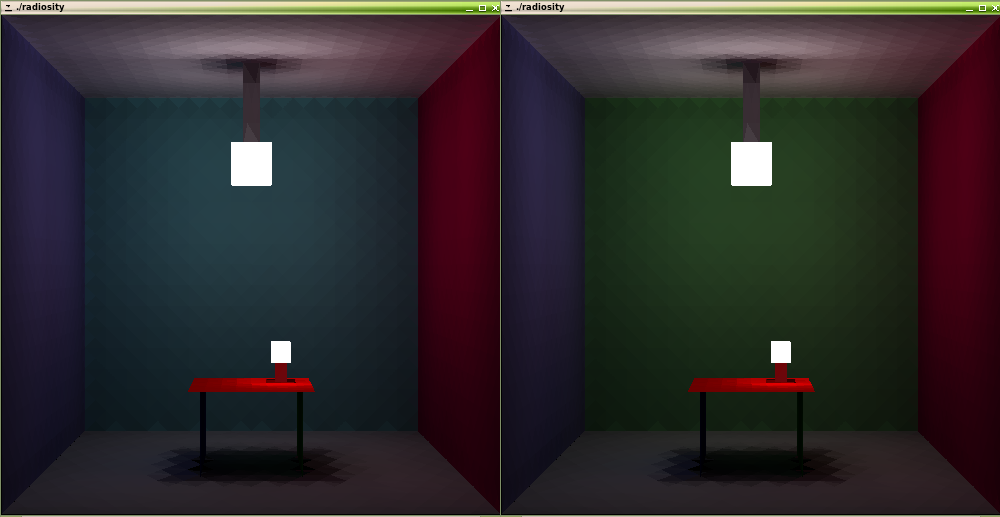
\includegraphics[width=12cm]{img/wrong_ff.png}
    \caption{Falsche Formfaktoren in den Ecken.}
    \label{fig:ff_corner}
  \end{figure}
  \begin{figure}[htb]
    \centering
    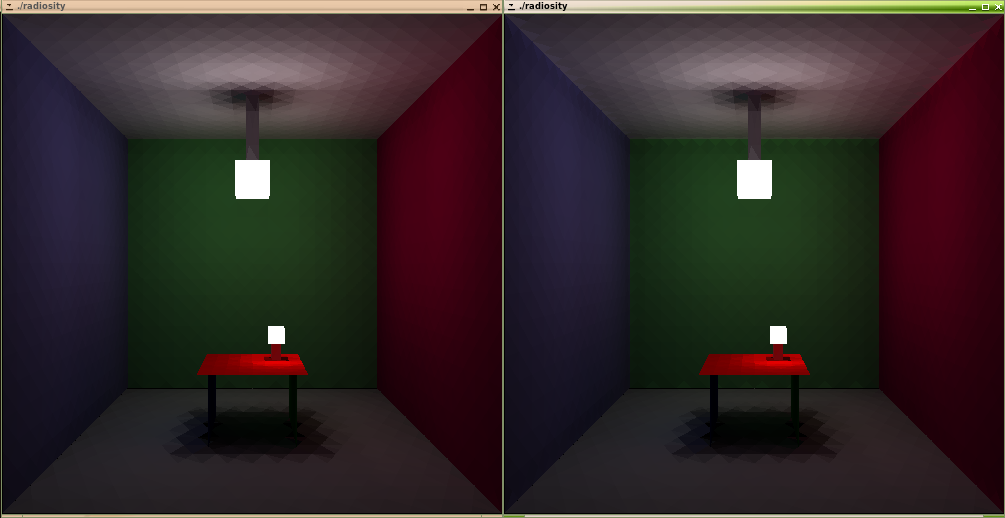
\includegraphics[width=12cm]{img/correct_ff.png}
    \caption{Links: falsche Formfaktoren, Rechts: korrigierte
    Formfaktoren.}
    \label{fig:ff_correct}
  \end{figure}
\end{appendix}
\end{document}
